\lstinputlisting[language=bash,basicstyle=\small]{python_codes/fieldstone_52/keywords}

\begin{center}
Code at \url{https://github.com/cedrict/fieldstone/tree/master/python_codes/fieldstone_52}
\end{center}

\par\noindent\rule{\textwidth}{0.4pt}

%%%%%%%%%%%%%%%%%%%%%%%%%%%%%%%%%%%%%%%%%%%%%%%%%%%%%%%%%%%%%%%%%%%%%%%%%%%%%%%%%%%%%%%

In order to test the grid point and connectivity algorithms, 
we use this simple $4\times 3$ element mesh:

\begin{verbatim}
      Q_2 X Q1 (serendipity)                    Q_2 X Q_1 (regular)

15--47--16--48--17--49--18--50--19      54--55--56--57--58--59--60--61--62
 |       |       |       |       |       |   :   |   :   |   :   |   :   |
42      43      44      45      46      45..46..47..48..49..50..51..52..53
 |       |       |       |       |       |   :   |   :   |   :   |   :   |
10--38--11--39--12--40--13--41--14      36--37--38--39--40--41--42--43--44
 |       |       |       |       |       |   :   |   :   |   :   |   :   |
33      34      35      36      37      27..28..29..30..31..32..33..34..35
 |       |       |       |       |       |   :   |   :   |   :   |   :   |
05--29--06--30--07--31--08--32--09      18--19--20--21--22--23--24--25--26
 |       |       |       |       |       |   :   |   :   |   :   |   :   |
24      25      26      27      28      09..10..11..12..13..14..15..16..17
 |       |       |       |       |       |   :   |   :   |   :   |   :   |
00--20--01--21--02--22--03--23--04      00--01--02--03--04--05--06--07--08

iel= 0:                                  iel= 0
node  0 : 0 at pos. 0.0 0.0              node  0 : 0 at pos. 0.0 0.0
node  1 : 1 at pos. 1.0 0.0              node  1 : 2 at pos. 1.0 0.0
node  2 : 6 at pos. 1.0 1.0              node  2 : 20 at pos. 1.0 1.0
node  3 : 5 at pos. 0.0 1.0              node  3 : 18 at pos. 0.0 1.0
node  4 : 20 at pos. 0.5 0.0             node  4 : 1 at pos. 0.5 0.0
node  5 : 25 at pos. 1.0 0.5             node  5 : 11 at pos. 1.0 0.5
node  6 : 29 at pos. 0.5 1.0             node  6 : 19 at pos. 0.5 1.0
node  7 : 24 at pos. 0.0 0.5             node  7 : 9 at pos. 0.0 0.5
                                         node  8 : 10 at pos. 0.5 0.5
\end{verbatim}

We see that the serendipity element-based mesh counts only 51 nodes, as
opposed to 63 for its counterpart.

Setting $nelx=nely$, we can look at the number of velocity nodes for each 
as a function of $nelx$, as shown hereunder:

\begin{center}
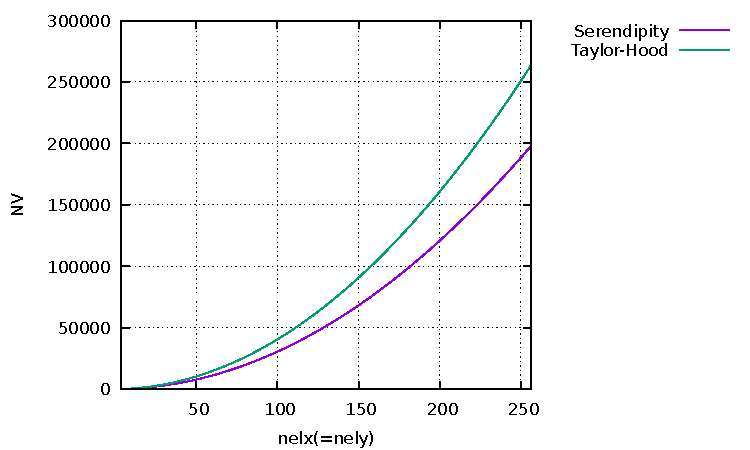
\includegraphics[width=6cm]{python_codes/fieldstone_52/images/NV.pdf}
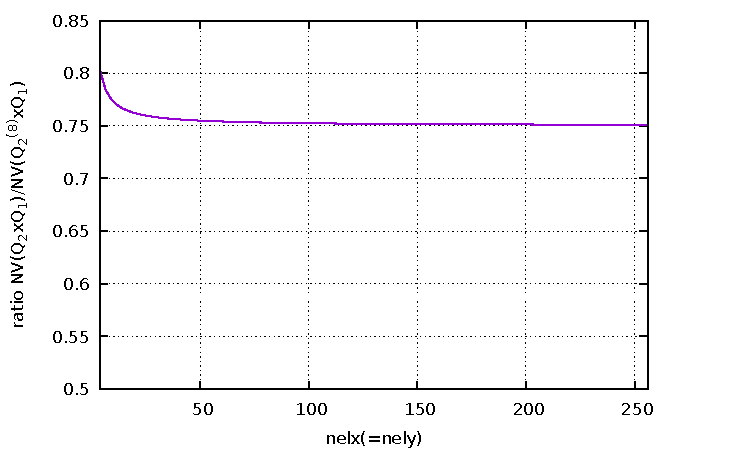
\includegraphics[width=6cm]{python_codes/fieldstone_52/images/NV_ratio.pdf}\\
{\captionfont Left: NV for both elements as a function of nelx. Right: ratio of the 
two.}
\end{center}
Looking at the ratio between both, we see that ultimately 
at high resolution, a mesh composed of serendipity elements 
will count 25\% less nodes than a mesh with Taylor-Hood elements.
Since there is not free lunch, what is the price paid in terms of accuracy when using 
the cheaper serendipity? 

The shape functions and their derivatives are in Section~\ref{sec:serendipity2D}.

Although the vtk format does not understand the $Q_2$ element in 2D or 3D, it surprisingly does
understand the serendipity element in 2D (type=23) and 3D (type=25).

\begin{center}
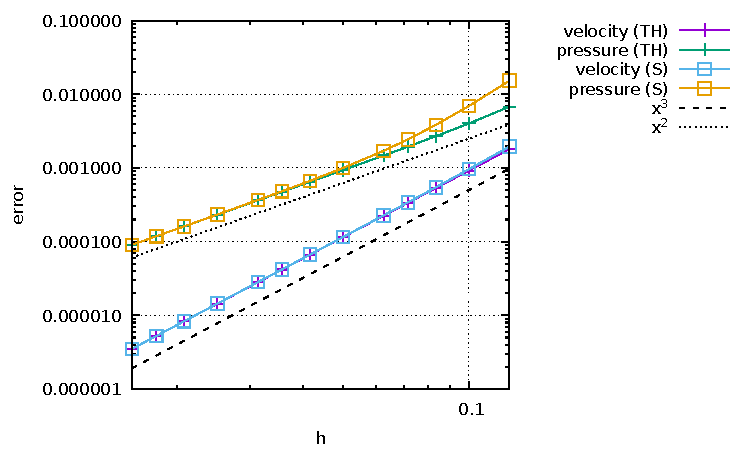
\includegraphics[width=8cm]{python_codes/fieldstone_52/images/errors.pdf}\\
{\captionfont 'TH' is Taylor-Hood. 'S' is serendipity.}
\end{center}

It looks like the serendipity element yields the same errors and error convergence 
rates as its Taylor-Hood counterpart. Since it is cheaper in terms of dofs, 
one could think that it should be preferred. However, most modern codes 
use an iterative solver approach to solve the discretised Stokes problem, and 
often the $\K$ matrix (which is SPD) is 'solved' with a conjugate gradient solver.  
The convergence of this type of solver depends on the condition number of the matrix
itself, i.e. the ratio of the largest and smallest eigenvalues. 
Note that this is rather trivial with Python:

\begin{lstlisting}
print('condition number:', nel,linalg.cond(K_mat))
\end{lstlisting}
However, since I was also curious about the values of the eigenvalues, I implemented 
it as follows:
\begin{lstlisting}
eigvals, eigvecs = linalg.eig(K_mat)
print('eigenvalues:',nel,eigvals.min(),eigvals.max())
\end{lstlisting}



\begin{center}
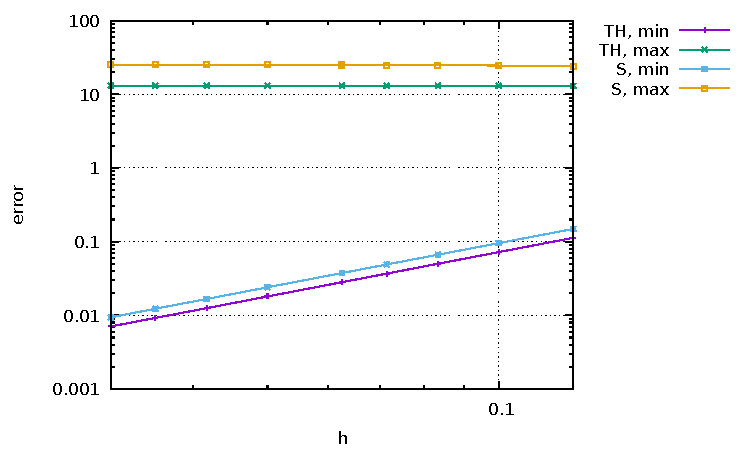
\includegraphics[width=6cm]{python_codes/fieldstone_52/images/eigenvalues.pdf}
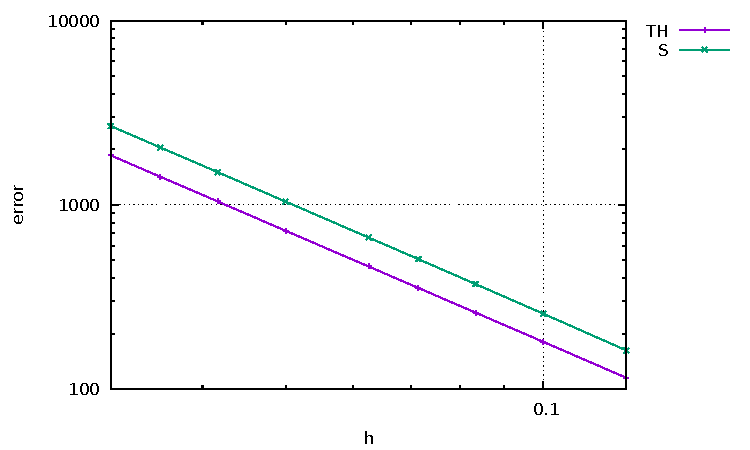
\includegraphics[width=6cm]{python_codes/fieldstone_52/images/eigenvalues_ratio.pdf}\\
{\captionfont Left: min and max eigenvalues for both types of elements as a function of $h$; 
Right: condition number}
\end{center}
As it turns out, the condition number is twice as high for the serendipity element, 
which means that the CG would have to iterate more to arrive at the solution, 
thereby offsetting the benefit of less dofs.





